\section{相关产品介绍及精度对比}
\subsection{\texorpdfstring{$p\mathrm{CO_2}$ }{}产品介绍}
\begin{table}[h]  
\centering  
\bicaption{\label{tab:不同产品对比}不同$p\mathrm{CO_2}$产品的对比}{Comparison of different $p\mathrm{CO_2}$ products}  
\begin{tabular}{M{0.18\textwidth} M{0.12\textwidth} M{0.23\textwidth} M{0.15\textwidth} M{0.15\textwidth}}  
\toprule % 使用booktabs宏包的\toprule命令生成更好的表格顶部线条  
产品      & 时间区域      & \multicolumn{1}{c}{输入变量}      & 回归方法      & 处理策略 \\ \midrule % 使用\midrule命令生成更好的表格中间线条 
CSIR-ML6 & 1980-2020    & \begin{tabular}[c]{@{}p{\dimexpr0.23\textwidth-2\tabcolsep\relax}@{}}SST, Chl-a, MLD\end{tabular} & 机器学习 & 低值替代 \\  
MPI-SOMFFN & 1998-2020 & \begin{tabular}[c]{@{}p{\dimexpr0.23\textwidth-2\tabcolsep\relax}@{}}SST, SSS, MLD, Chl-a, $x\mathrm{CO_2}$\end{tabular} & 神经网络 & 忽略Chl-a \\  
LSCE-FNN & 2001-2016 & \begin{tabular}[c]{@{}p{\dimexpr0.23\textwidth-2\tabcolsep\relax}@{}}SSS, SST, MLD, Chl-a, $x\mathrm{CO_2}$, SSH\end{tabular} & 神经网络 & 低值替代 \\  
JAM-MLR & 1993–2018 & \begin{tabular}[c]{@{}p{\dimexpr0.23\textwidth-2\tabcolsep\relax}@{}}SST, SSS, MLD, SSDH, Chl-a\end{tabular} & 线性回归 & 忽略Chl-a \\  
% NIES-FNN & 1990-2018 & \begin{tabular}[c]{@{}p{\dimexpr0.23\textwidth-2\tabcolsep\relax}@{}}Mon, LAT, LON, SST, SSS, Chl-a\end{tabular} & 神经网络 & 低值替代 \\  
% NIES3 & 1980-2020 & \begin{tabular}[c]{@{}p{\dimexpr0.23\textwidth-2\tabcolsep\relax}@{}}SST, SST anomaly, SSS, Chl-a, MLD, LAT, LON, year\end{tabular} & 机器学习 & 低值替代 \\ 
\bottomrule % 使用\bottomrule命令生成更好的表格底部线条  
\end{tabular}  
\end{table} 

在1.3小节中,我们介绍了一些关于全球$p\mathrm{CO_2}$的研究进展,这些研究都取得了不错的研究成果,为我们初步理解全球$p\mathrm{CO_2}$的时空变化提供了帮助。然而大部分研究都提到,南大洋地区存在很大的分歧或不确定性\cite{CSIR_ML6,MPI_SOMFFN,socat2016}。我们分析这可能是由于冬季叶绿素数据缺失引起的,因此,我们选择了SOCCOM项目中收录的多种机器学习方法的产品进行对比。这些产品有着较多的共性,比如:都是以SOCAT数据集中提供的$p\mathrm{CO_2}$为目标变量,同时也使用了相似的输入变量,并都采用了回归方法。如\autoref{tab:不同产品对比}所示,列举的这些产品都以全球$p\mathrm{CO_2}$为研究对象,且都提供了月平均$p\mathrm{CO_2}$产品,但分辨率较低,仅为1°×1°。

虽然这些产品取得了不错的成果,但是他们在处理冬季高纬度Chl-a缺失问题上仍然存在着一些不完美,这些产品在处理该问题的策略大体上分为两类:一是使用假设值(低值)替代,如CSIR-ML6\cite{CSIR_ML6}、LSCE-FNN\cite{LSCE_FFNN}等产品,例如CSIR-ML6产品假设$log(\mathrm{Chl-a})=0$来填补缺失的叶绿素,LSCE-FNN产品则也是假设低值,且加上了一定的噪声;另一种策略是直接忽略叶绿素,如MPI-SOMFNN产品\cite{MPI_SOMFFN}和JMA-MLR产品\cite{JMA_MLR}在冬季无叶绿素的地区只使用剩余的环境变量进行回归拟合,这无疑会加剧冬季估算的不确定性。
% 、NIES-FNN\cite{zeng2022surface}、NIES3\cite{zeng2014global};NIES3产品则是使用了气候态叶绿素来填补

这些假设方法与真实情况有差距,或多或少都对$p\mathrm{CO_2}$的准确反演造成了一定的干扰。并且考虑到各产品在计算$\mathrm{CO_2}$通量过程中可能使用了不同的风速、温度产品,为了更清晰地比较各产品的碳汇量区别,我们对各产品的$\mathrm{CO_2}$通量重新进行了计算。在此过程中,我们仅使用了各产品中的$p\mathrm{CO_2}$数据,确保了其他变量的一致性,以便进行最后的对比。

\subsection{独立航次精度对比}
\begin{figure}[htbp]
    \centering
    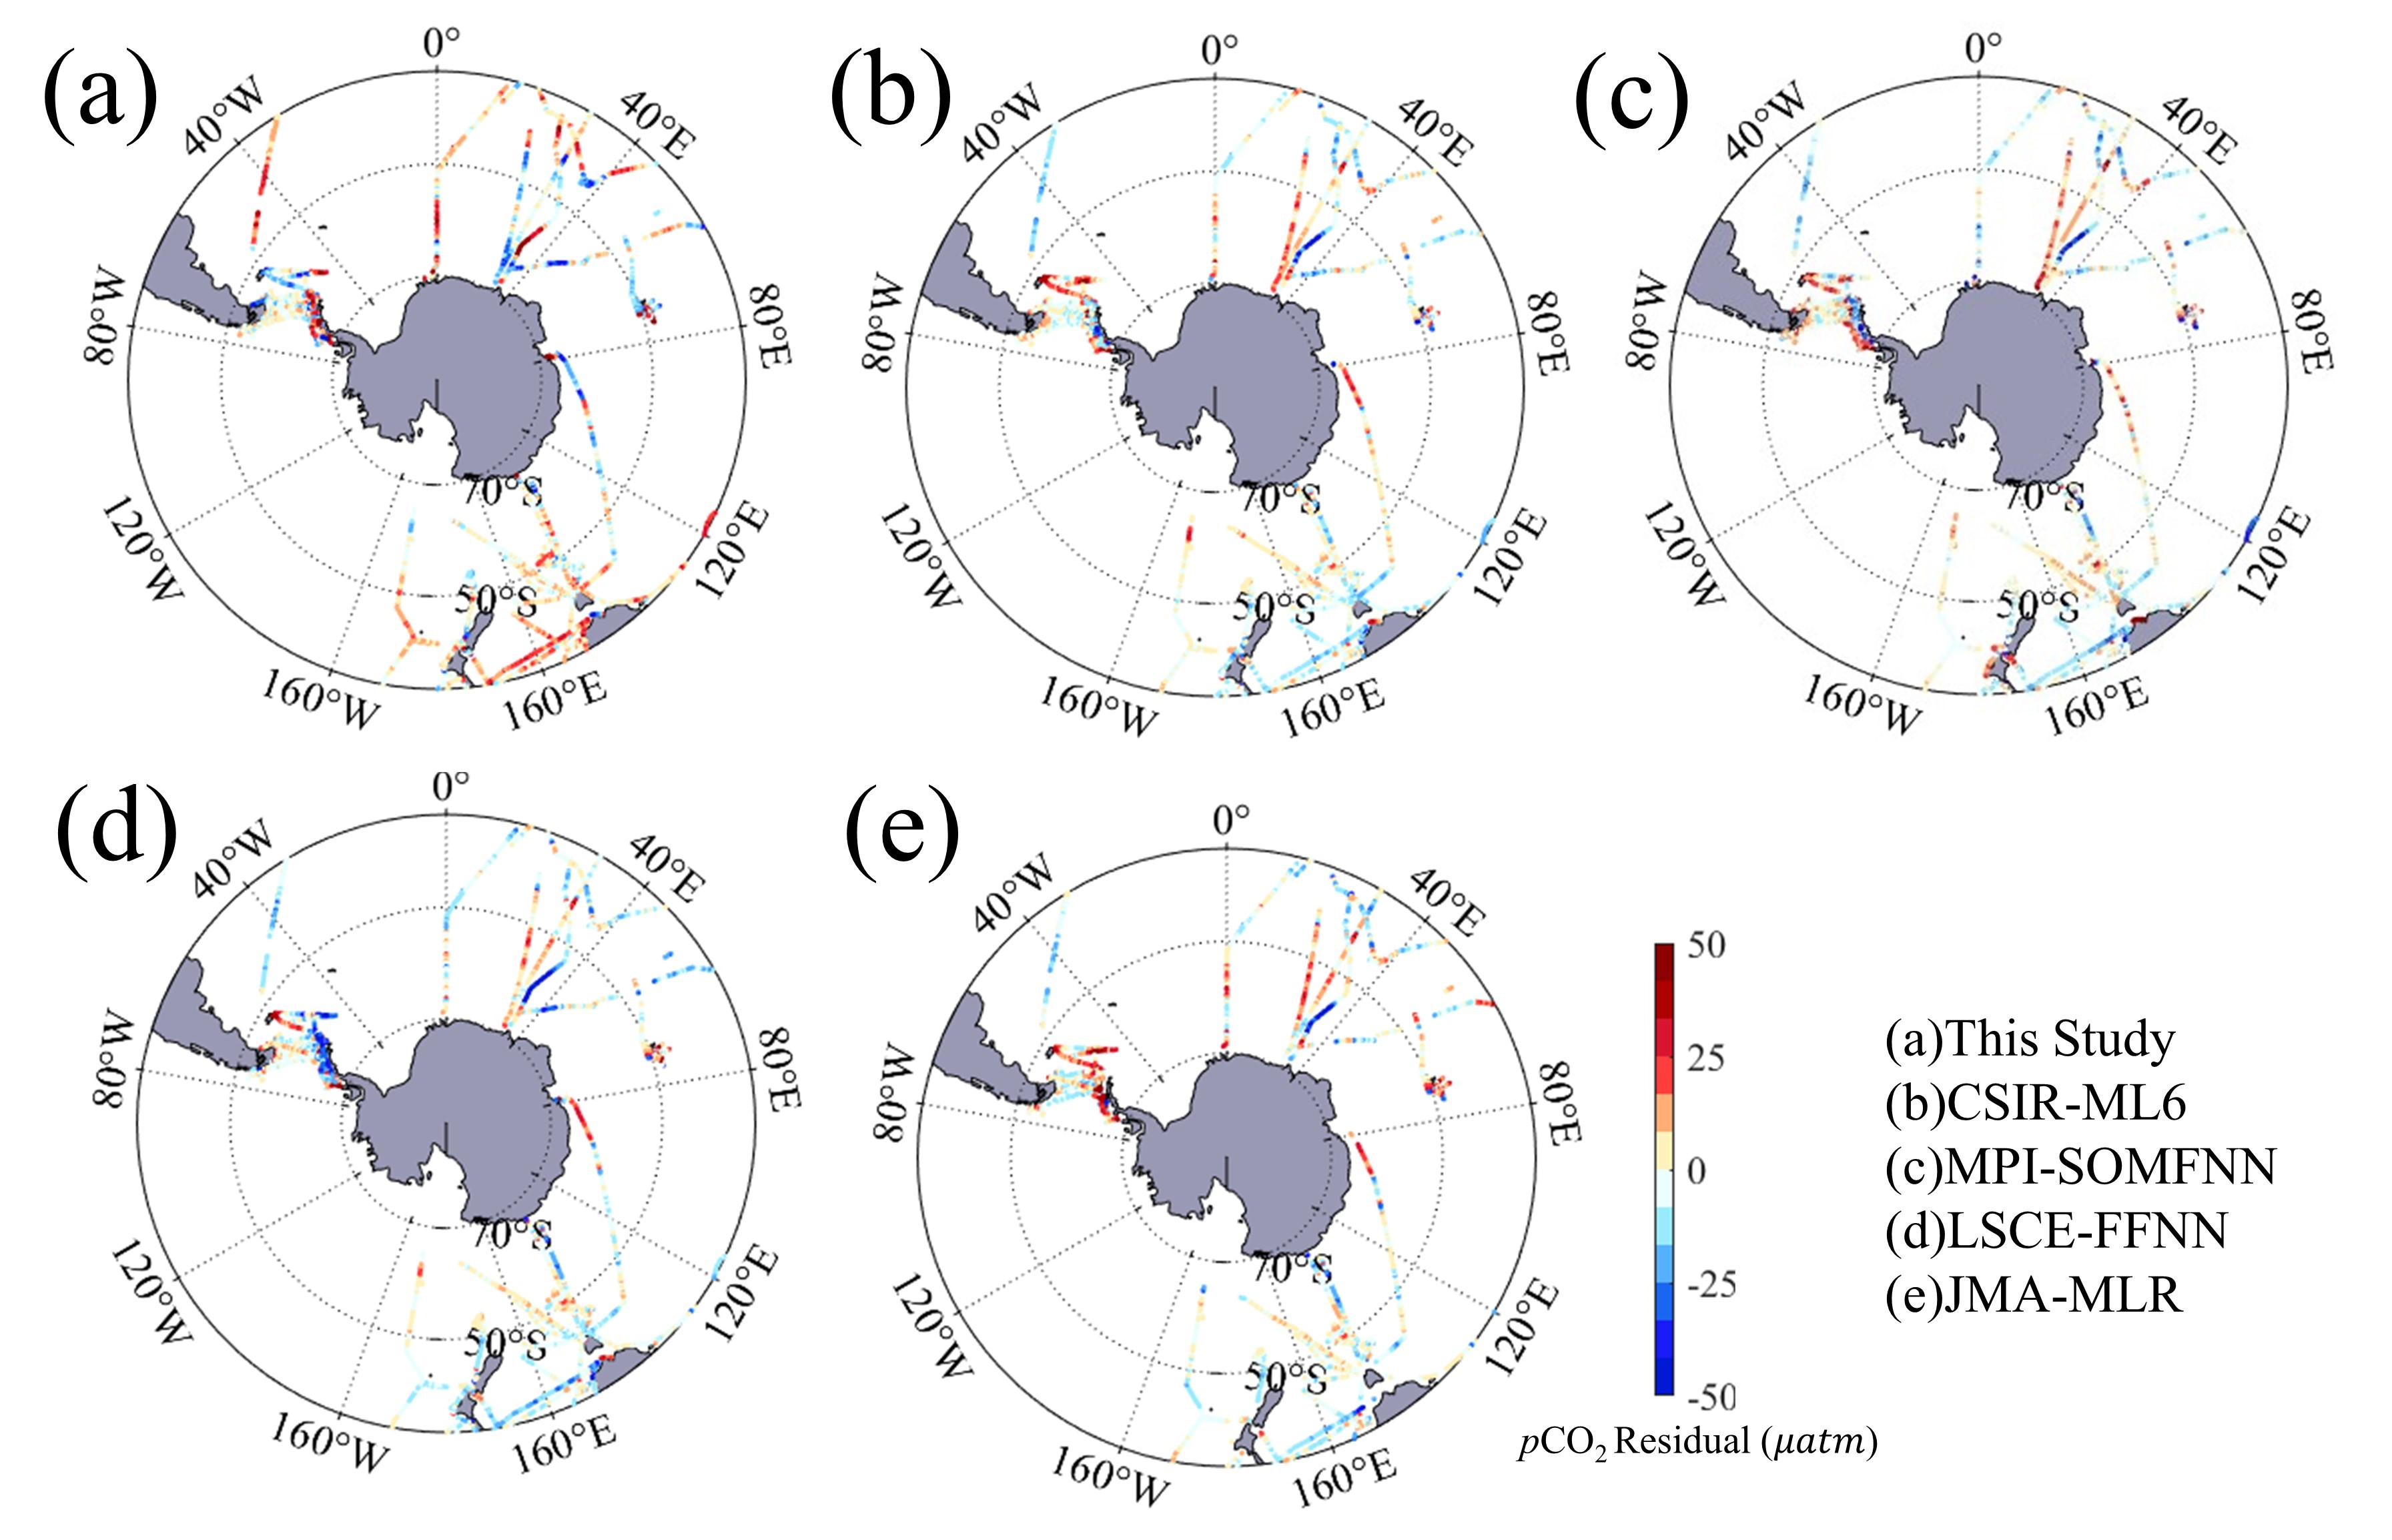
\includegraphics[width=\linewidth]{figure/第四章用图/精度对比.jpg}
    \bicaption{\label{fig:精度对比}独立航次在不同数据产品中的精度对比}
    {Precision comparison of independent voyage in different data products  }
\end{figure}

在进行模型精度验证时,我们预留了五十条航次的数据进行独立测试,这里我们同样对比了这些数据与各产品月平均数据的残差值,结果如\autoref{fig:精度对比}和\autoref{tab:精度对比}所示。结果表明,这五种产品的精度表现相近,RMSE均在18μatm附近,MAE均在13左右,$\mathrm{R^2}$均在0.5左右。

且高纬度地区的残差值与低纬度残差相近,说明模型能够用于高纬度的反演。另外,对比产品匹配的为1°×1°月平均$p\mathrm{CO_2}$产品,相对来说,我们产品的结果在空间分辨率上有所提升。

\begin{table}[htbp]
\centering
\bicaption{\label{tab:精度对比}独立航次在不同数据产品中的精度对比}{Precision comparison of independent voyage in different data products}
\begin{tabularx}{\textwidth}{@{}lcccccc@{}}
\toprule
区域                      & 属性               & 本研究   & CSIR-ML6 & MPI-SOMFFN & LSCE-FFNN & JMA-MLR \\ \midrule
\multirow{4}{*}{南大洋}    & N\#              & 6623  & 6526     & 6594       & 6515      & 5003    \\
                        & RMSE  & 18.43 & 16.26    & 17.84      & 18.19     & 15.49   \\
                        & MAE              & 12.88 & 10.85    & 12.01      & 11.62     & 10.75   \\
                        & R2               & 0.52  & 0.60     & 0.54       & 0.53      & 0.56    \\ \midrule
\multirow{4}{*}{低纬度} & N\#              & 3033  & 2966     & 3013       & 2964      & 2056    \\
                        & RMSE  & 14.89 & 12.77    & 16.14      & 13.11     & 10.61   \\
                        & MAE              & 10.96 & 8.99     & 11.15      & 9.16      & 8.02    \\
                        & R2               & 0.51  & 0.65     & 0.40       & 0.63      & 0.69    \\  \midrule
\multirow{4}{*}{高纬度} & N\#              & 3590  & 3560     & 3581       & 3551      & 2947    \\ 
                        & RMSE  & 20.20 & 18.47    & 18.98      & 21.67     & 18.29   \\
                        & MAE              & 14.31 & 12.37    & 12.72      & 13.84     & 12.81   \\
                        & R2               & 0.44  & 0.53     & 0.53       & 0.41      & 0.40    \\ \bottomrule 
\end{tabularx}
\end{table}

\section{南大洋\texorpdfstring{$p\mathrm{CO_2}$ }{}时空变化}
在第三章中,我们通过详细的研究和经历多次训练过程,成功地构建了一个能够可靠稳定地反演南大洋$p\mathrm{CO_2}$的XGBoost模型(XGB模型)。这个模型不仅准确度高,而且运行效率也相当出色。我们将利用这个模型,使用输入变量的月平均数据来反演出南大洋月平均$p\mathrm{CO_2}$分布情况。最终得到了2008年1月-2016年12月的月平均$p\mathrm{CO_2}$分布情况。如\autoref{fig:fig-4pCO2空间分布}所示,(a)图显示了本模型反演出的$p\mathrm{CO_2}$和其他产品在南大洋整个区域的月平均变化时间序列。同时,(b)和(c)图则分别展示了低纬度区域和高纬度区域情况,进一步揭示了南大洋中不同区域的$p\mathrm{CO_2}$分布和变化情况。

总的来说,研究时间内,南大洋的$p\mathrm{CO_2}$呈现了缓慢上升趋势和显著的季节变化特征。如\autoref{fig:fig-4pCO2时间变化}所示,月平均$p\mathrm{CO_2}$从2008年1月的354.45μatm增加到2016年12月的365.14μatm,南大洋的$p\mathrm{CO_2}$平均增加速率为1.88μatm yr$^{-1}$,而如\autoref{fig:fig-4pCO2时间变化}-(a)中的虚线所示,大气中$p\mathrm{CO_2}$的增加率为2.14μatm yr$^{-1}$,这说明南大洋的$\Delta p\mathrm{CO_2}$在增加,可推测出南大洋的碳汇也在增加。南大洋的$p\mathrm{CO_2}$季节特征尤为显著,所有产品都表现出一致的季节变化,夏季达到最低,冬季达到最高。值得注意的是,多数产品在冬季的最高值明显高于我们的结果。从低纬度(\autoref{fig:fig-4pCO2时间变化}-(b))和高纬度(\autoref{fig:fig-4pCO2时间变化}-(c))的时间序列图中可以看到,其他产品在低纬度的夏季和高纬度的冬季可能都存在高估的情况。

\begin{figure}[htbp]
    \centering
    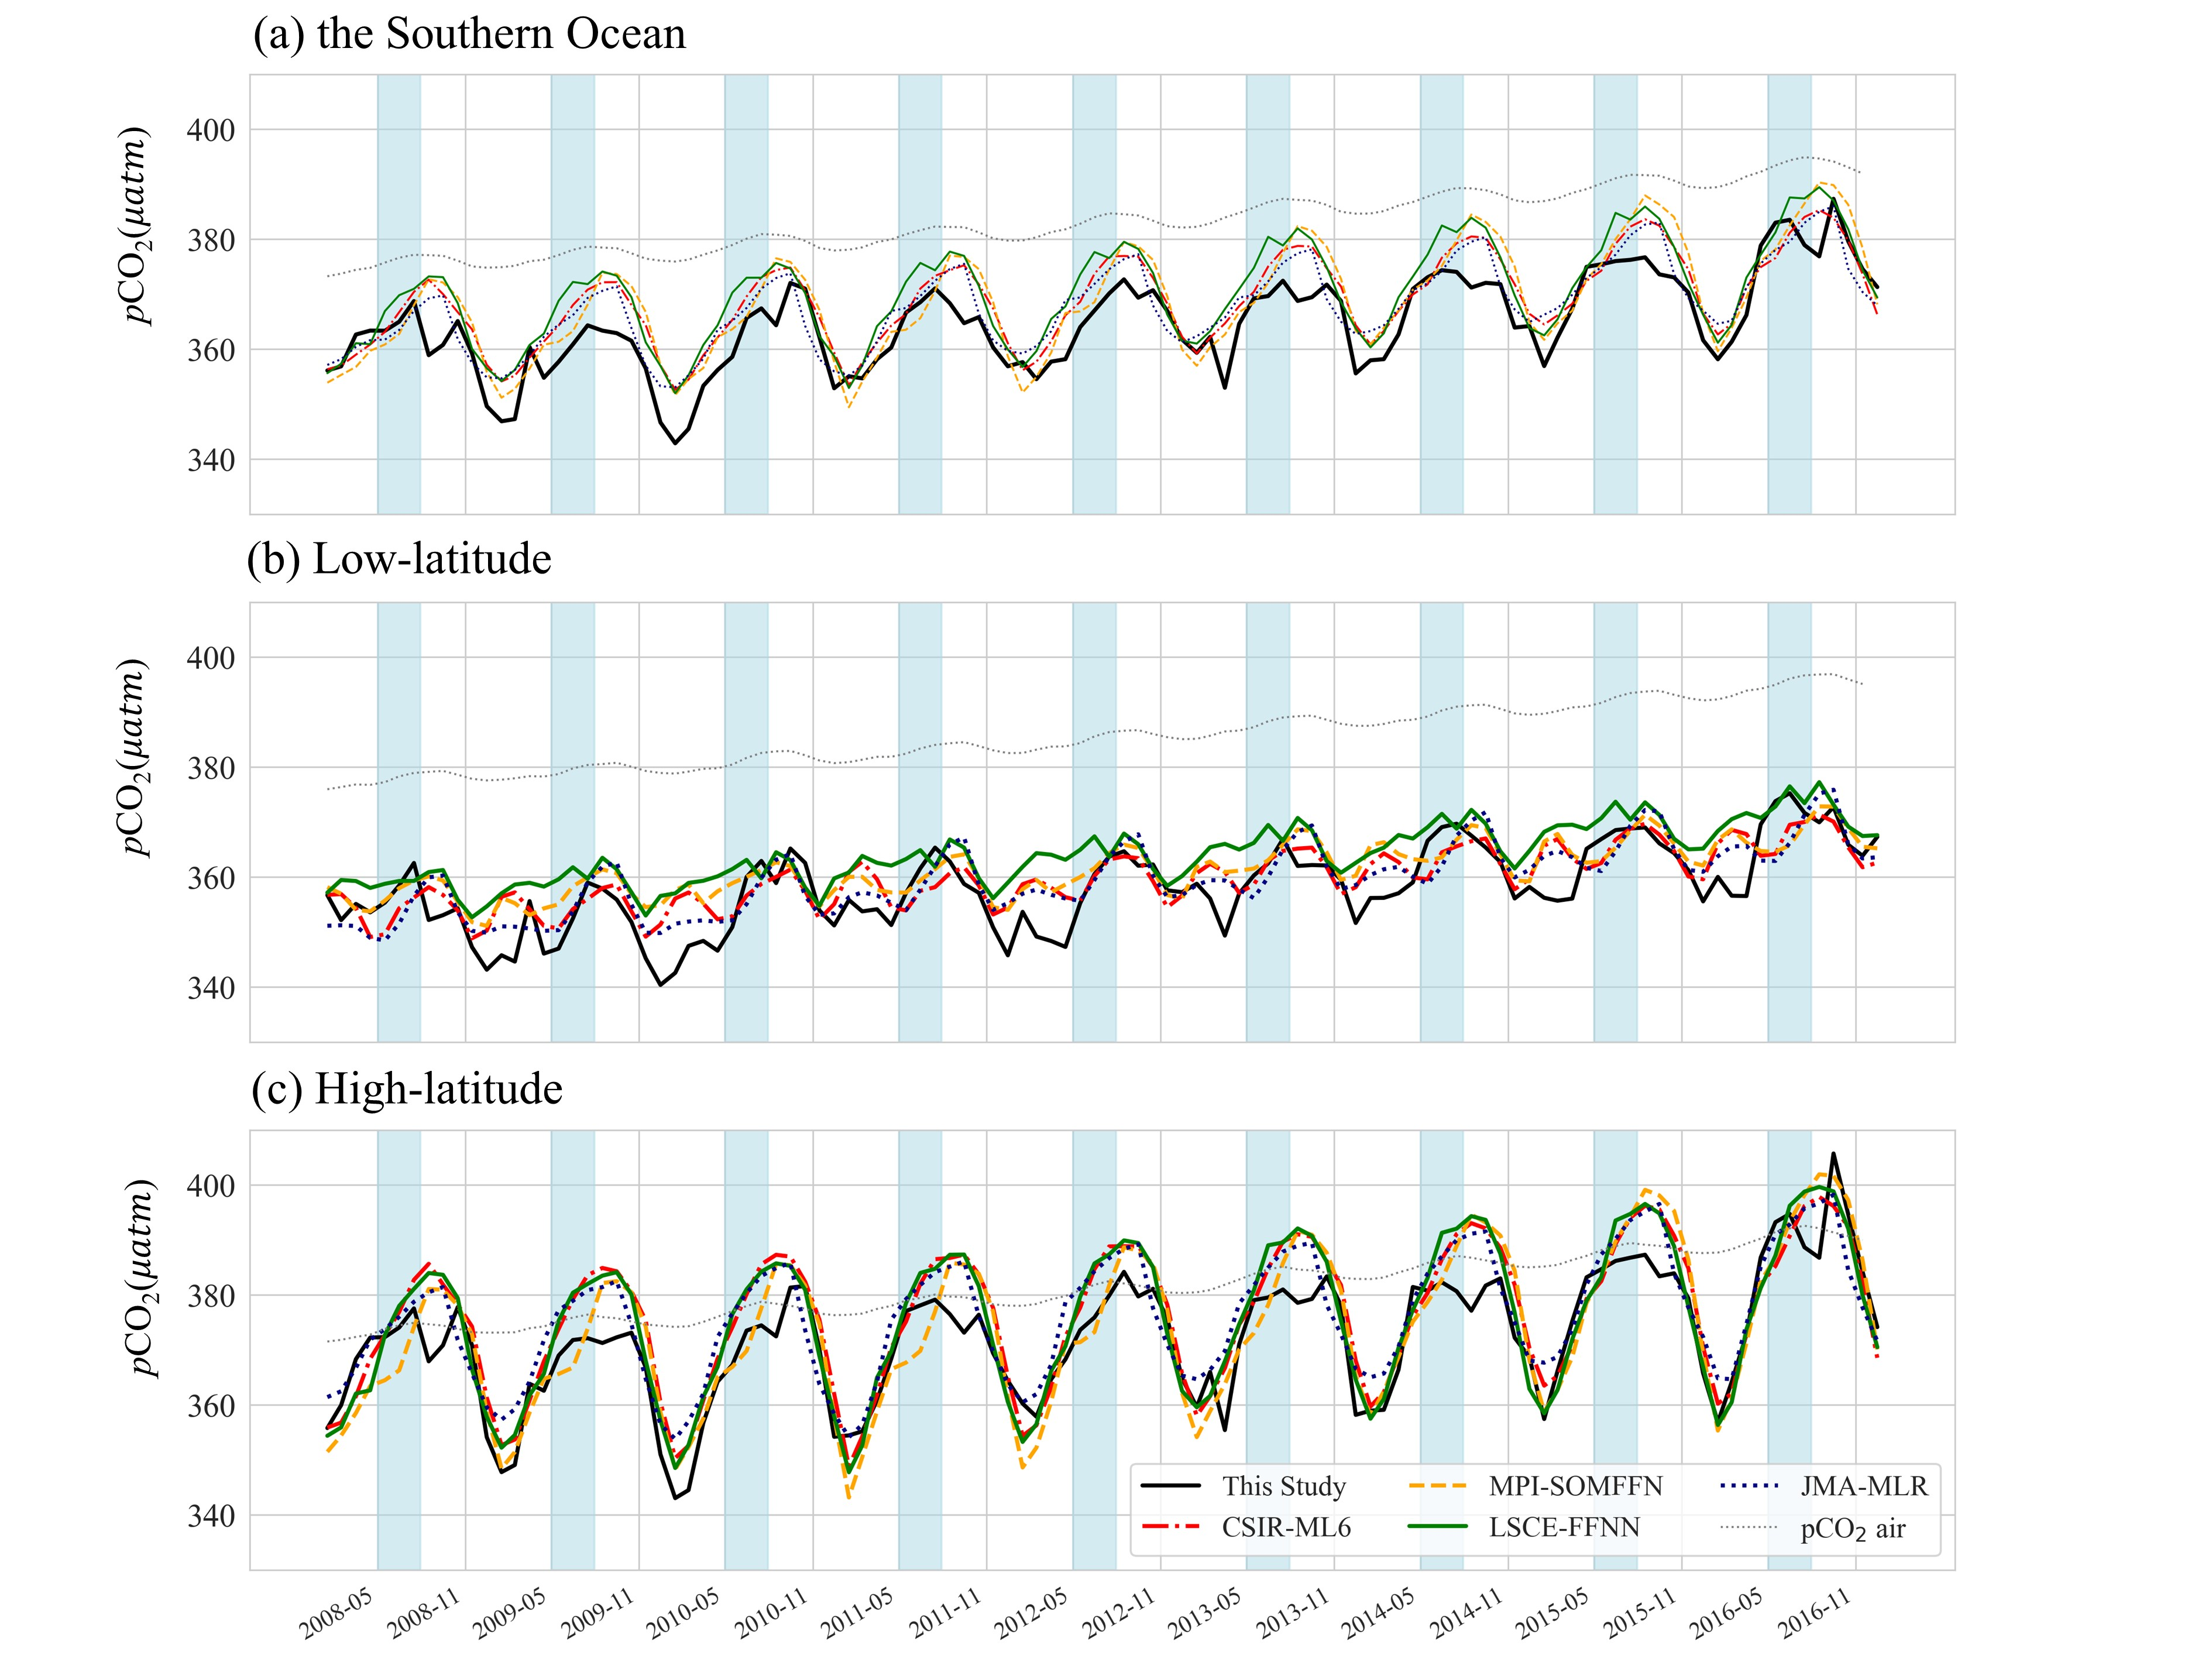
\includegraphics[width=1.1\linewidth]{figure/第四章用图/图4-pCO2.jpg}
    \bicaption{\label{fig:fig-4pCO2时间变化}(a)各产品中的南大洋月平均$p\mathrm{CO_2}$时间序列,(b)、(c)分别为低纬度和高纬度地区各产品月平均$p\mathrm{CO_2}$时间序列}
    {(a) The monthly average $p\mathrm{CO_2}$ time series for each product in the Southern Ocean, and (b) and (c) are the monthly average $p\mathrm{CO_2}$ time series for each product at low and high latitudes, respectively}
\end{figure}

如\autoref{fig:fig-4pCO2空间分布}所示,从$p\mathrm{CO_2}$空间分布情况来看,南大洋在夏秋季节有较为明显的分布特征,呈现为“双环结构”。即STSS区域和Ice区域是低值集中区,而SPSS区域是高值集中区,这可能是由于生物等因素的影响。然而,在春季和冬季,分布特性并不明显,具体表现为越往南,$p\mathrm{CO_2}$值越高。产品间对比可发现他们的数据覆盖面积存在差异,比如MPIS-SOMFFN产品能覆盖到全部非陆地区域,而其他产品则没有。这是由于各产品可能使用了不同的冰浓度产品和叶绿素处理策略,因此在计算flux时,我们统一了冰浓度产品以确保永久冰层区域不参与统计。其次,在春季和冬季,高纬度地区的$p\mathrm{CO_2}$值大小差异最为明显。

\begin{figure}[htbp]
    \centering
    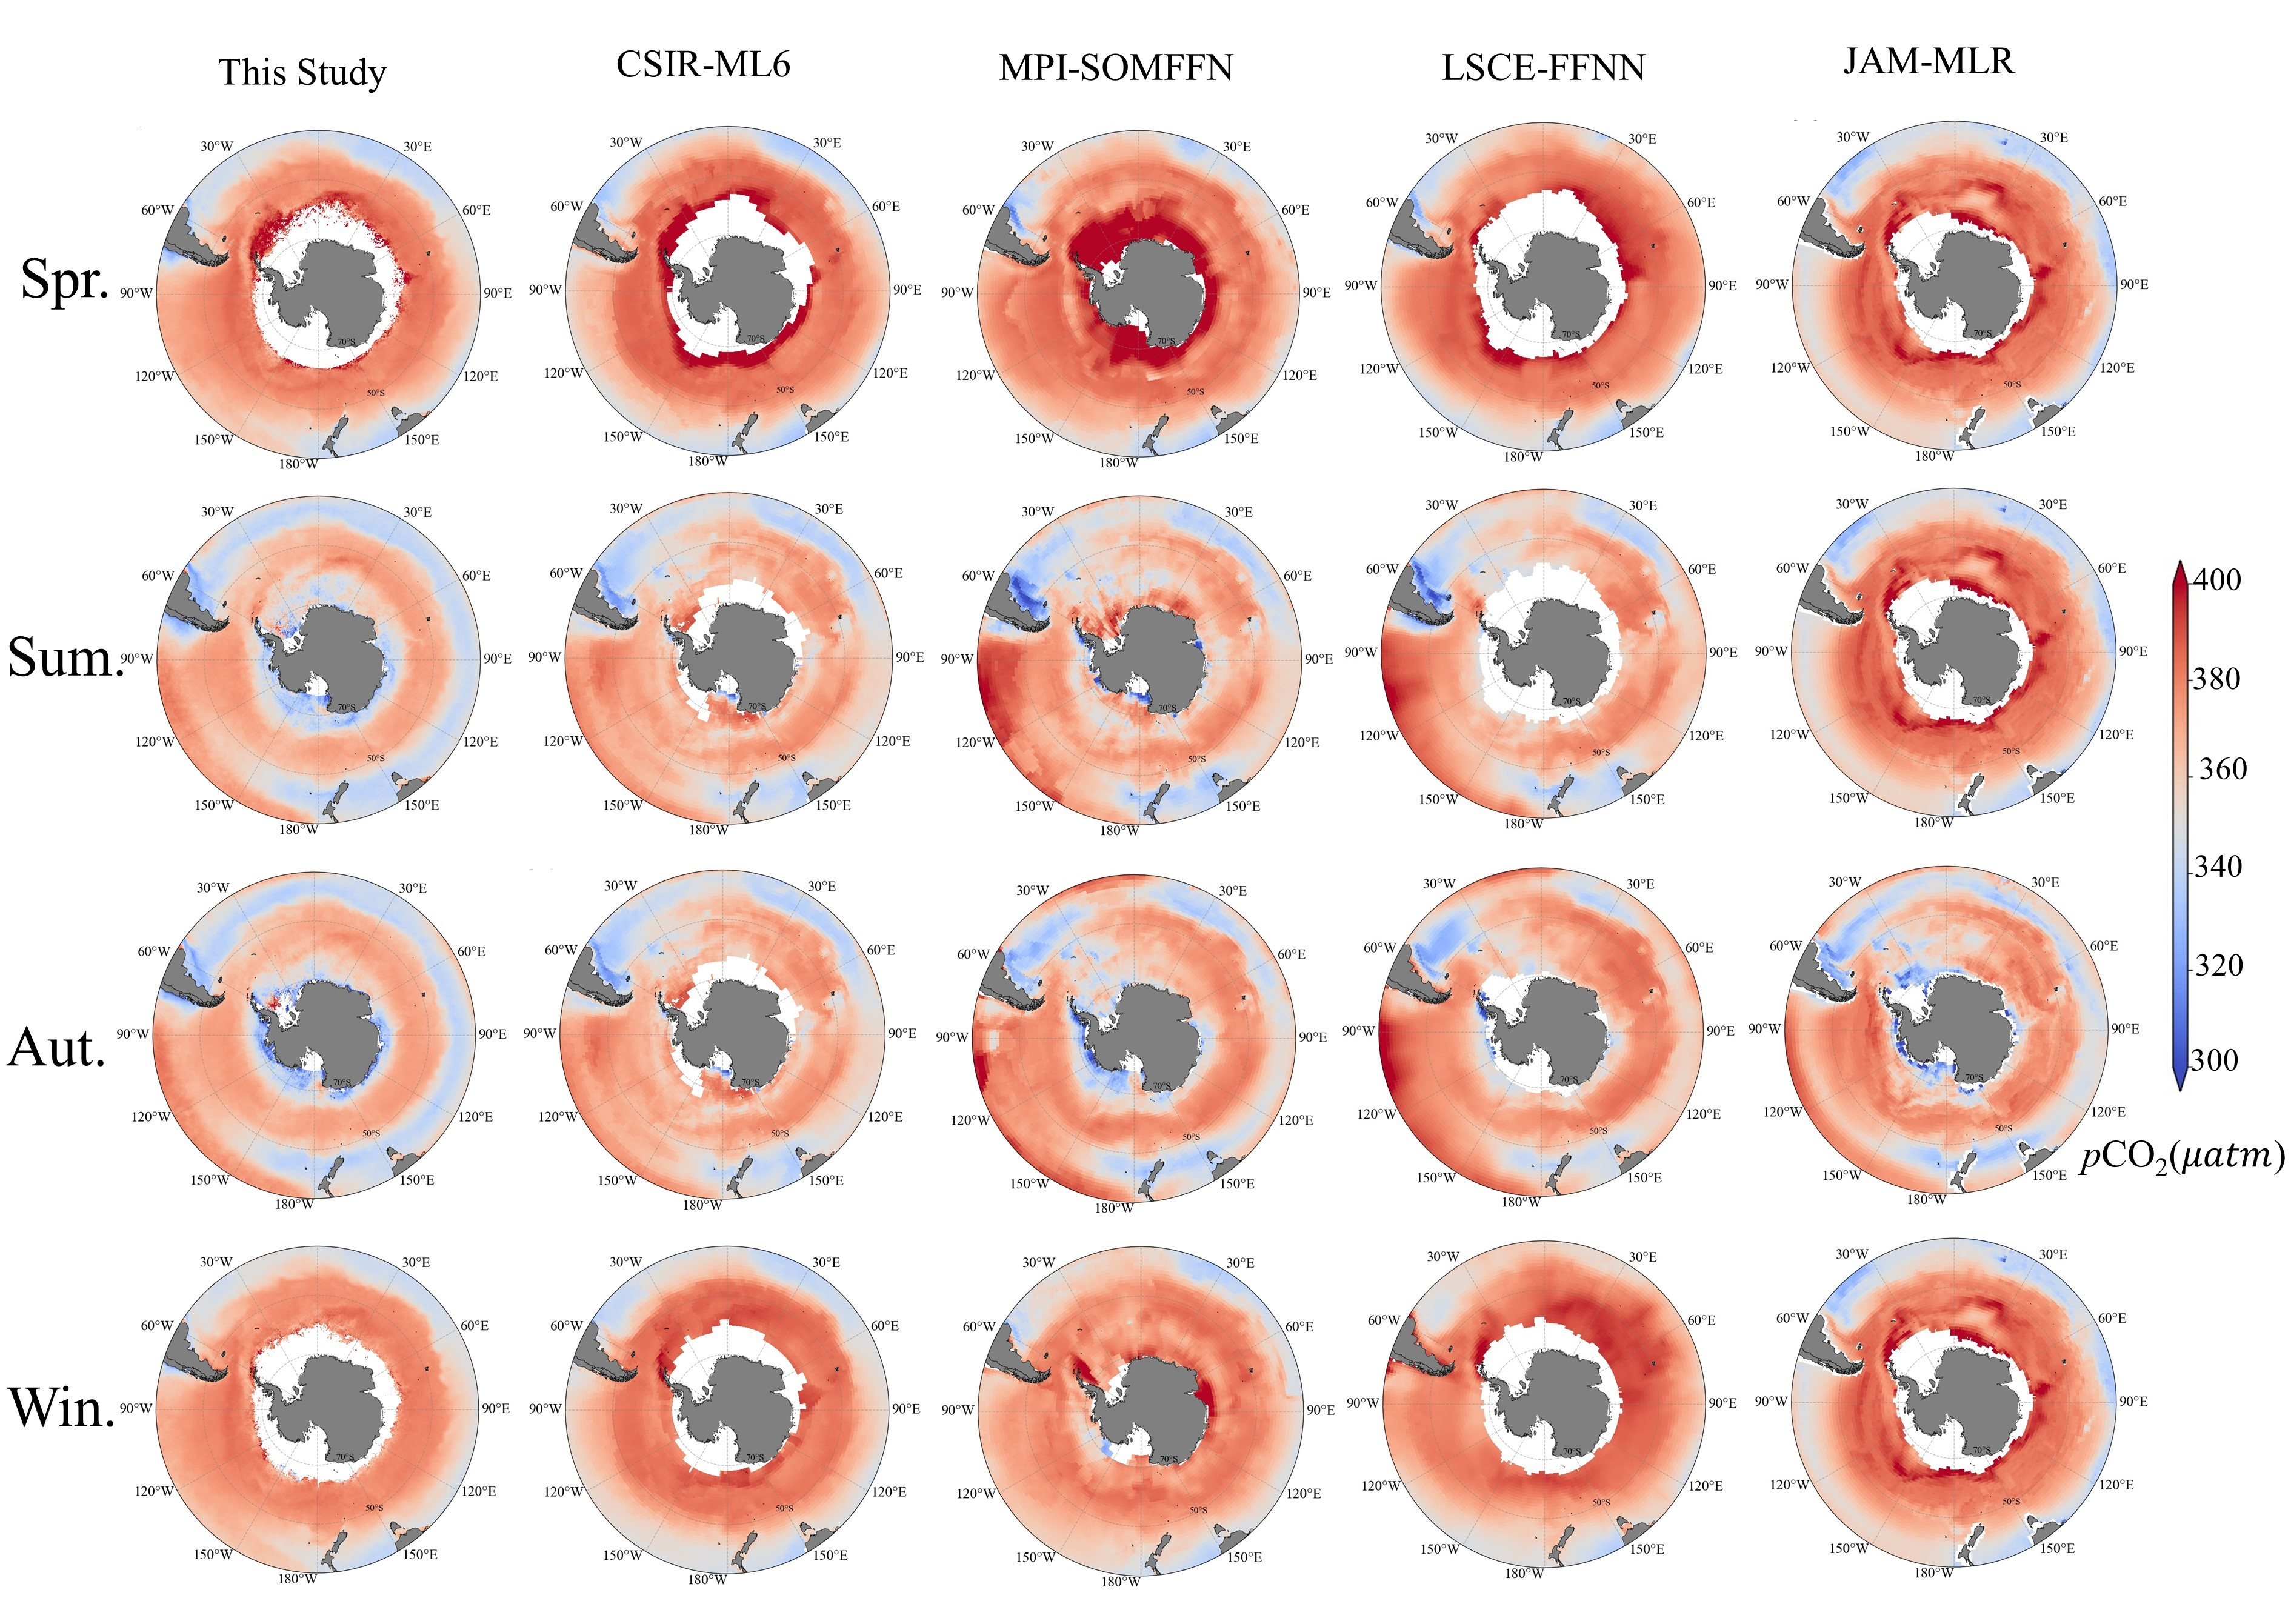
\includegraphics[width=\linewidth]{figure/第四章用图/图4-pCO2分布.jpg}
    \bicaption{\label{fig:fig-4pCO2空间分布}(a)各产品南大洋季节平均$p\mathrm{CO_2}$空间分布,(b)、(c)分别为低纬度和高纬度地区各产品季节平均$p\mathrm{CO_2}$空间分布}
    {(a) the seasonal average $p\mathrm{CO_2}$spatial distribution of each product in the Southern Ocean, (b) and (c) are the seasonal average $p\mathrm{CO_2}$spatial distribution of each product in low and high latitudes, respectively}
\end{figure}

\section{南大洋碳汇时空变化}
\subsection{南大洋海-气\texorpdfstring{$\mathrm{CO_2}$}{}通量的计算}
南大洋碳汇作为海洋生态系统的重要组成部分,通过吸收大气中的$\mathrm{CO_2}$,不仅能够减缓全球变暖的速度,还有助于维持海洋生态系统的稳定性和多样性。为了量化海洋吸收能力的强弱,我们量化了研究区域内的海-气$\mathrm{CO_2}$交换通量$\mathrm{CO_2}$\ $flux$来分析南大洋碳汇变化趋势。$\mathrm{CO_2}$\ $flux$的单位为$mmol \cdot m^{-2}day^{-1}$,计算公式为:
% $$
% flux = k_w \times sol \times (p\mathrm{CO_2^{sea}}-p\mathrm{CO_2^{air}})\times (1-ice)
% $$
\begin{equation}
    \label{equ:flux-1}
    flux = k_w \times sol \times (p\mathrm{CO_2^{sea}}-p\mathrm{CO_2^{air}})\times (1-ice)
\end{equation}
式中$K_w$是$\mathrm{CO_2}$气体传输速度,单位是$cm \ h^{-1}$,而$sol$是$\mathrm{CO_2}$在海水中的溶解度,单位为$mol\ m^{-3} \mu atm^{-1}$,主要受到了盐度、压强和温度的影响,这里计算过程参考了weiss等人\cite{weiss1974carbon}。其中$K_w$的计算公式参考了Wanninkhof等人\cite{wanninkhof2014relationship}的方法:
\begin{equation}
    \label{equ:flux-2}
    K_w=a\times<u^2>\times\left(Sc/660\right)^{-0.5}
\end{equation}
$a$ 是气体传输规模系数,在Fay等人\cite{Harmonization_2021}的研究中提到,它来源于气体交换过程的研究,与大气和海洋中$^{14}C$的含量有关。因此使用不同的风速数产品,$a$的值选择是有差异的。$u^2$是第二瞬时平均风速,过程中我们使用的是CCMP数据产品,对应a值为0.251\cite{Harmonization_2021}。
Sc为施密特数,其取决于表层海水的温度,其计算公式为:
\begin{equation}
    \label{equ:flux-3}
    S_c=2116.8-136.25\cdot T +4.7353\cdot  T^2-0.092307 \cdot T^3+0.0007555\cdot T^4
\end{equation}
最后考虑到季节性冰区的影响,最后$\mathrm{CO_2} flux$乘以权重(1-ice)以量化冰层对碳吸收的影响。

\subsection{南大洋碳汇时空特征}
\begin{figure}[htb]
    \centering
    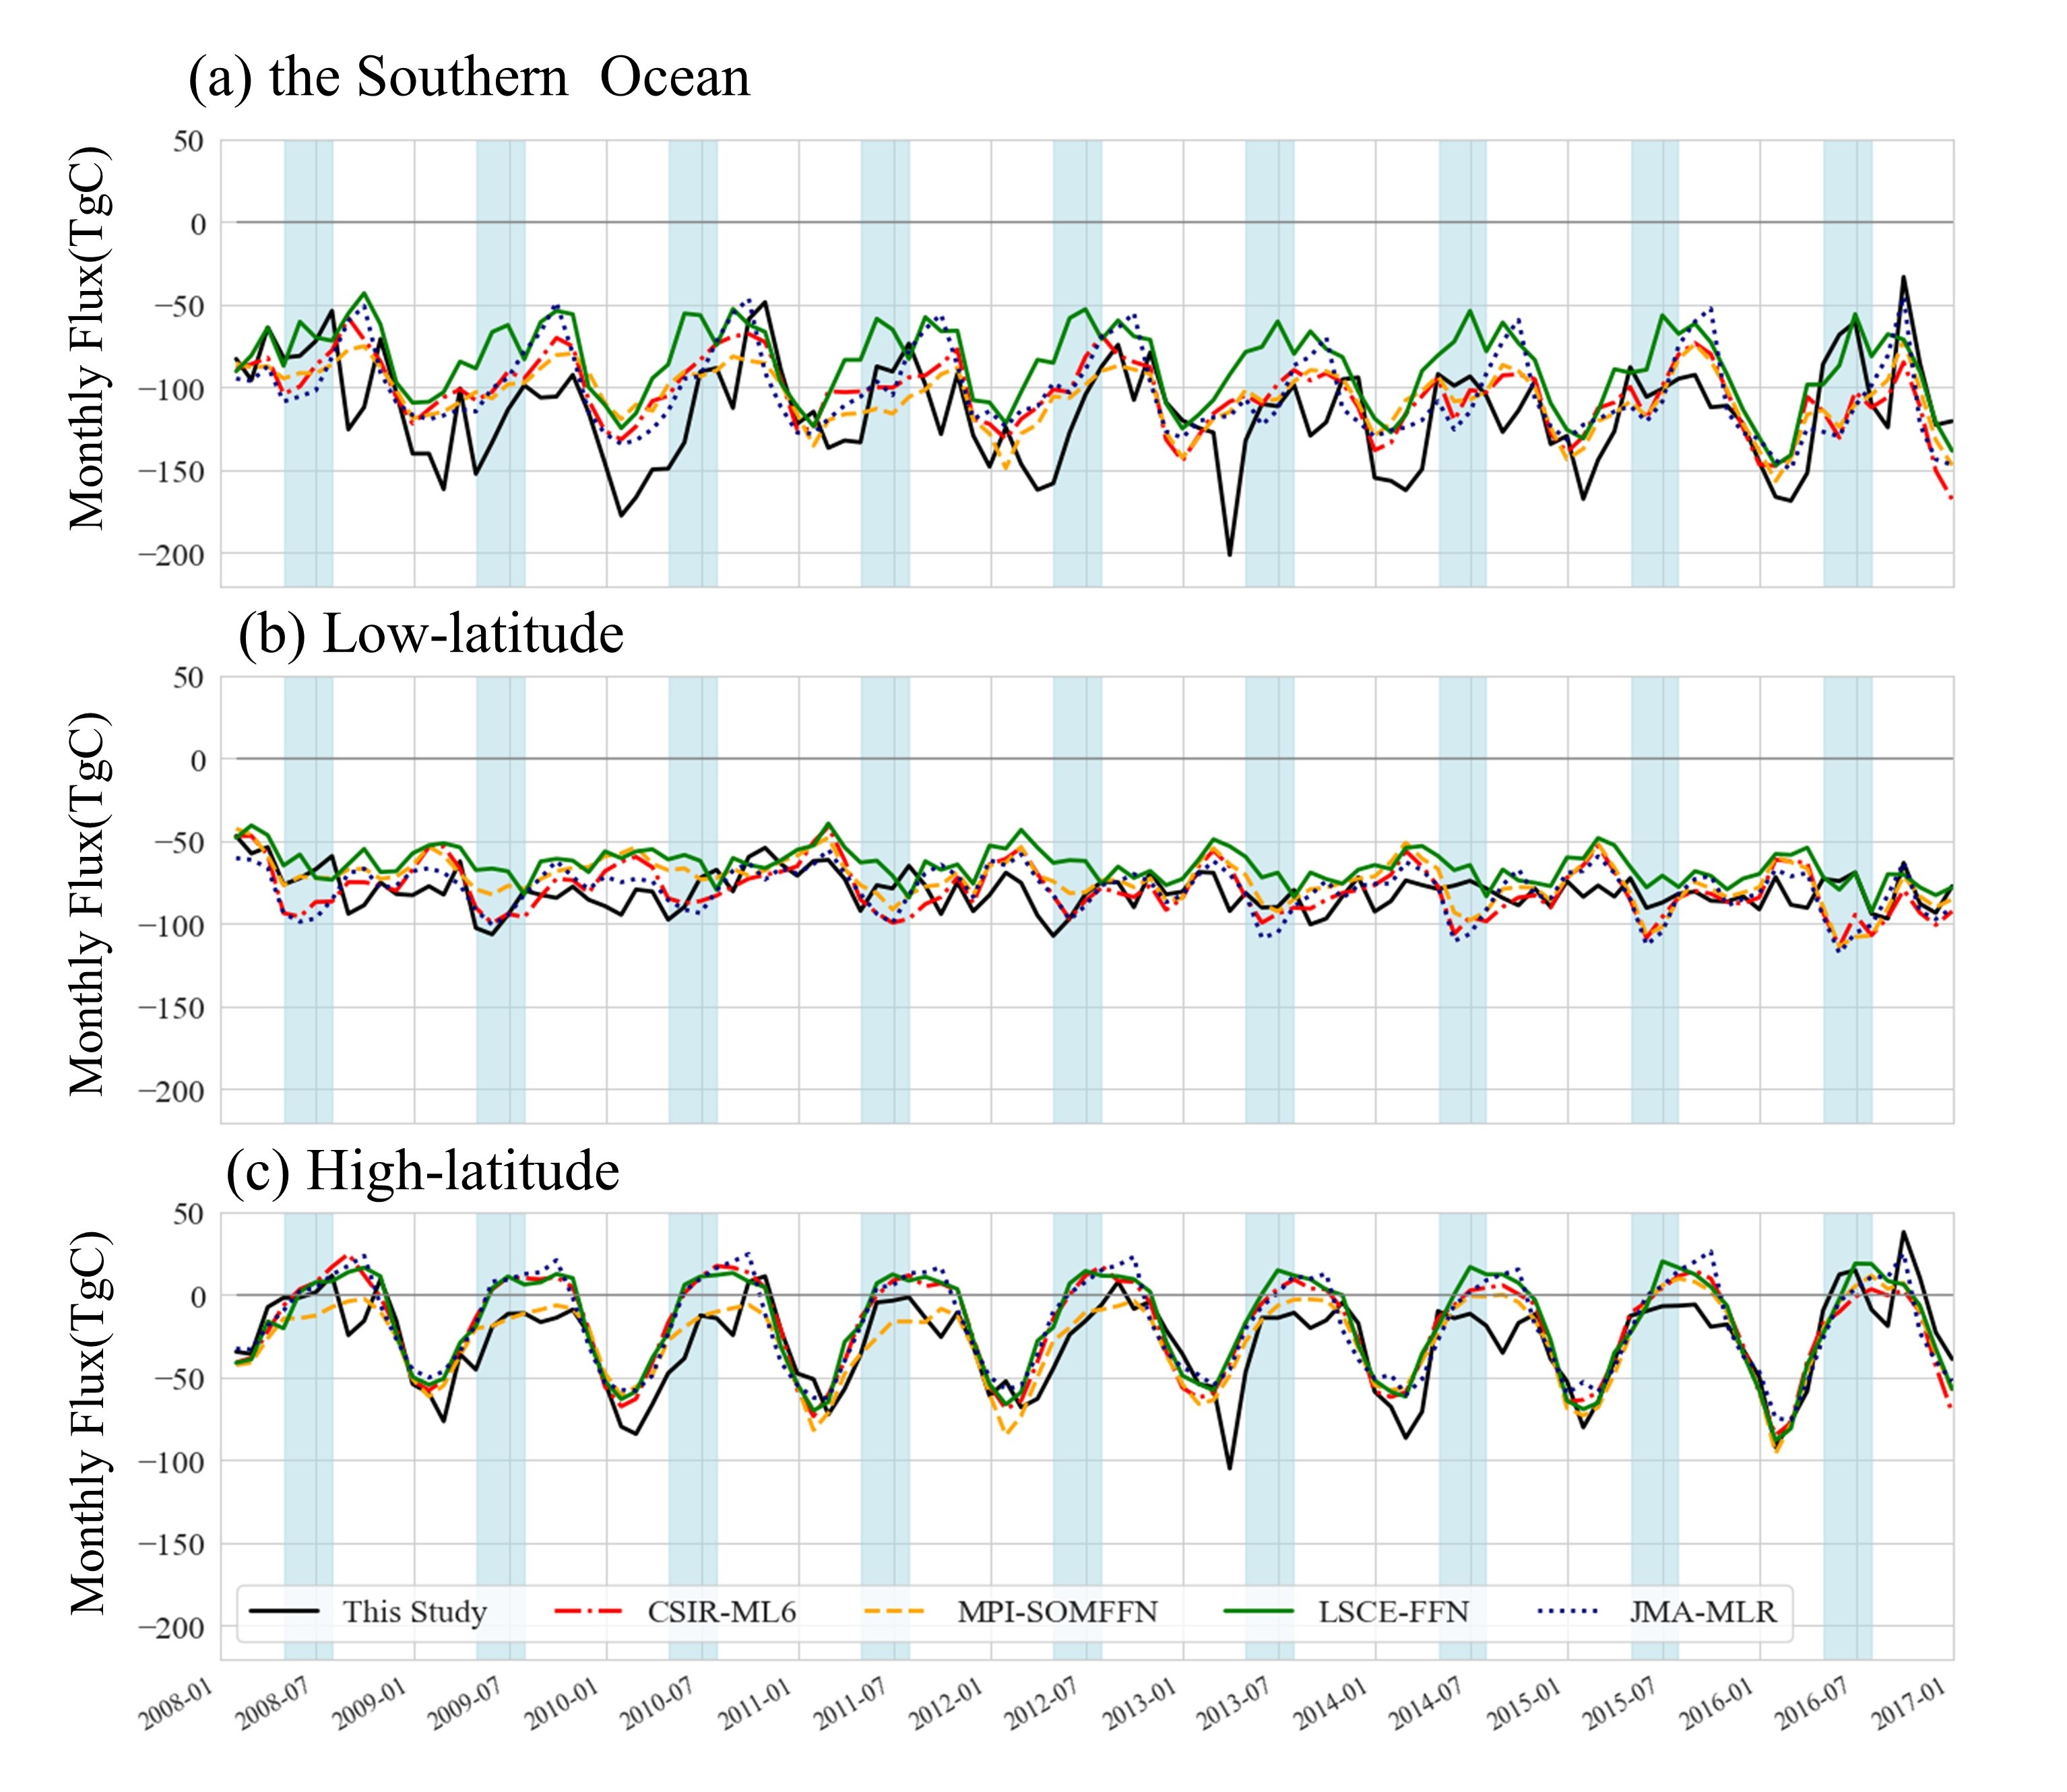
\includegraphics[width=\linewidth]{figure/第四章用图/图4-flux时间变化.jpg}
    \bicaption{\label{fig:fig-4flux时间变化}(a)各产品南大洋每月$\mathrm{CO_2}$ 通量时间序列,(b)、(c)分别为低纬度和高纬度地区各产品每月$\mathrm{CO_2}$ 通量时间序列}
    {(a) The monthly  $\mathrm{CO_2}$ flux time series for each product in the Southern Ocean, and (b) and (c) are the monthly  $\mathrm{CO_2}$ flux time series for each product at low and high latitudes, respectively}
\end{figure}

根据4.2.1小节的计算结果,我们得到了南大洋每月海气$\mathrm{CO_2}$交换通量的数据。如\autoref{fig:fig-4flux时间变化}所示,图(a)展示了整个南大洋区域的$\mathrm{CO_2}$吸收情况。可以看出,在研究期间南大洋一直在吸收$\mathrm{CO_2}$,并且每年以微弱的增幅增长,约为0.016Pg\ C\ yr$^{-1}$。图中还可以看出,南大洋在冬季的吸收量最少,这可能是温度影响了气体交换。根据图(b)和(c),我们可以知道南大洋的主要碳汇区域仍然集中在低纬度的STPS和STSS区域,而高纬度区域则有较为明显的季节变化,在冬季吸收最少,并且有多个产品认为是碳源区域。从整个区域的年平均来看,南大洋的碳汇量约为1.37±0.04Pg\ C\ yr$^{-1}$;其中,低纬度地区约吸收了0.96±0.02Pg\ C\ yr$^{-1}$的$\mathrm{CO_2}$,高纬度地区约吸收了0.35±0.03Pg\ C\ yr$^{-1}$的$\mathrm{CO_2}$。

如\autoref{fig:fig-4flux空间变化}所示,从空间分布来看,STSS区域是南大洋吸收碳主要的区域。这可能由于富含碳的深层水的影响。从整个区域来看,只有春季和冬季靠近冰域的少数地区是$\mathrm{CO_2}$释放区,这与比较的产品和之前的研究一致,多数研究归结于深层富含营养的海水上涌所导致。与其他产品相比,可以明显地发现这些产品在该区域存在$\mathrm{CO_2}$排放高估的情况。
\begin{figure}[htbp]
    \centering
    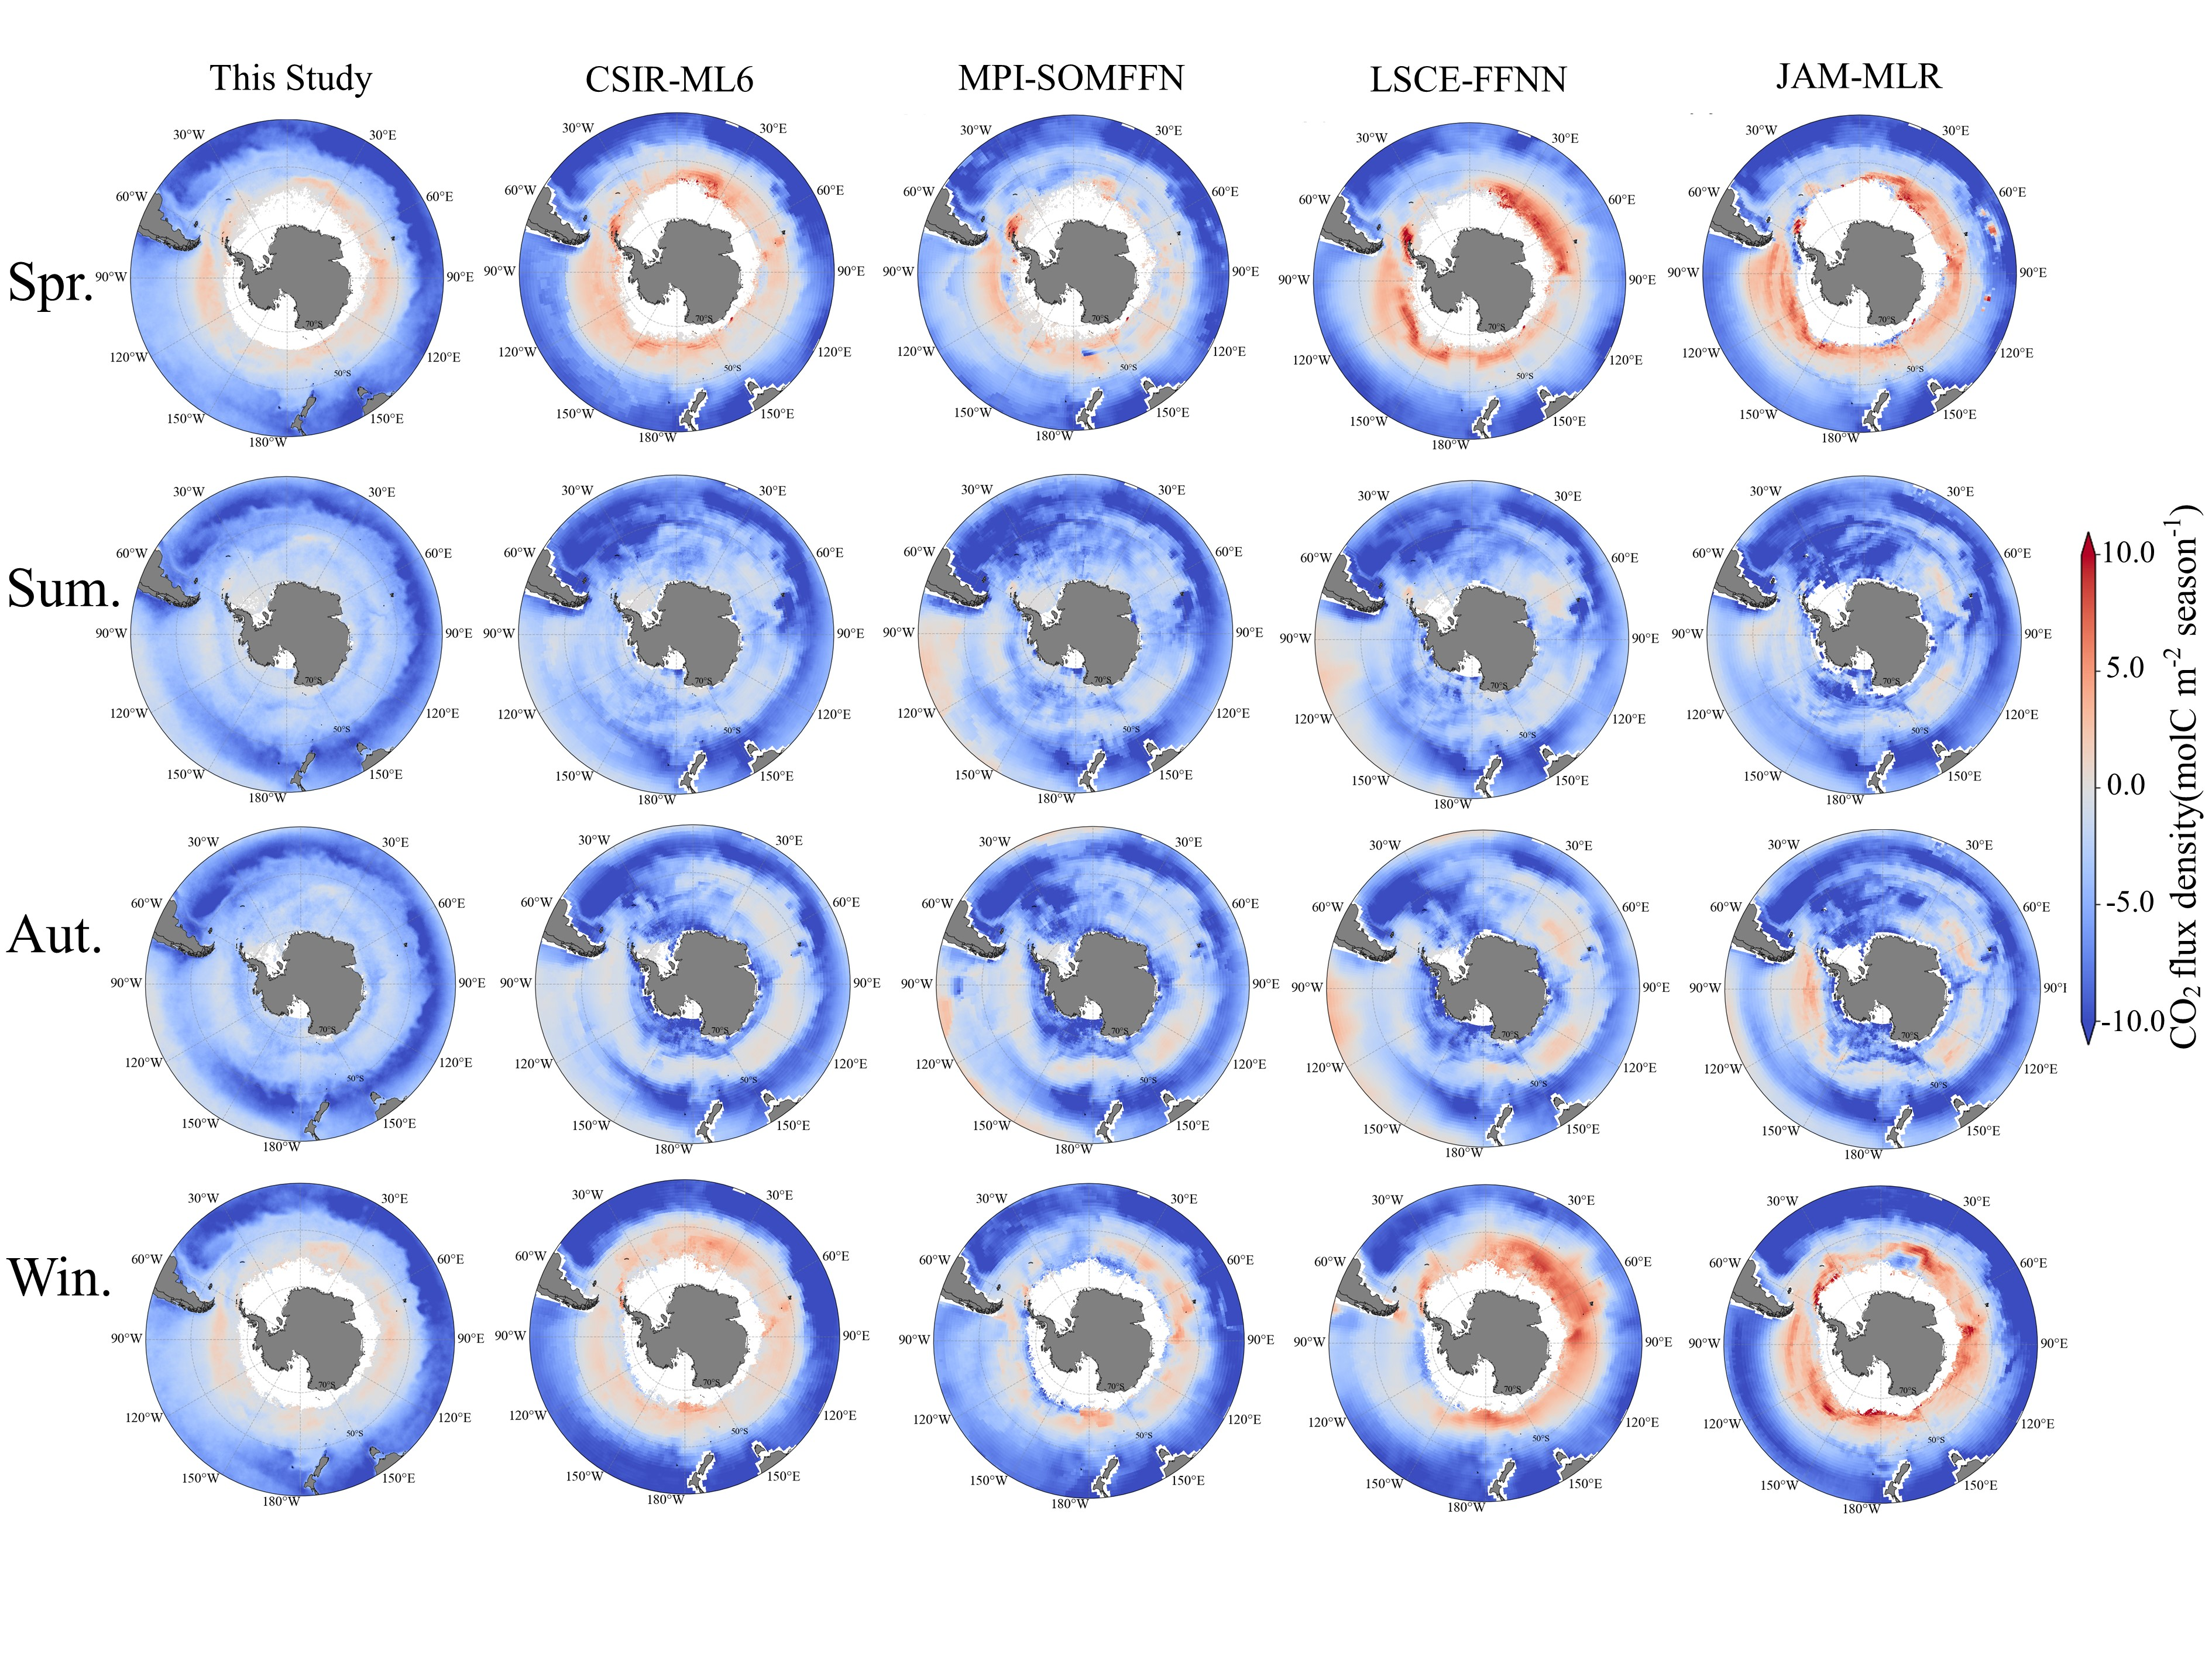
\includegraphics[width=\linewidth]{figure/第四章用图/图4-flux空间分布.jpg}
    \bicaption{\label{fig:fig-4flux空间变化}(a)各产品南大洋每月$\mathrm{CO_2}$ flux 密度分布图,(b)、(c)分别为低纬度和高纬度地区各产品每月$\mathrm{CO_2}$ flux 密度分布图}
    {(a) The monthly $\mathrm{CO_2}$ flux density distribution of each product in the Southern Ocean; (b) and (c) are the monthly $\mathrm{CO_2}$ flux density distribution of each product at low and high latitudes, respectively}
\end{figure}

\section{南大洋高纬度地区碳汇差异原因分析}

\begin{figure}[htbp]
    \centering
    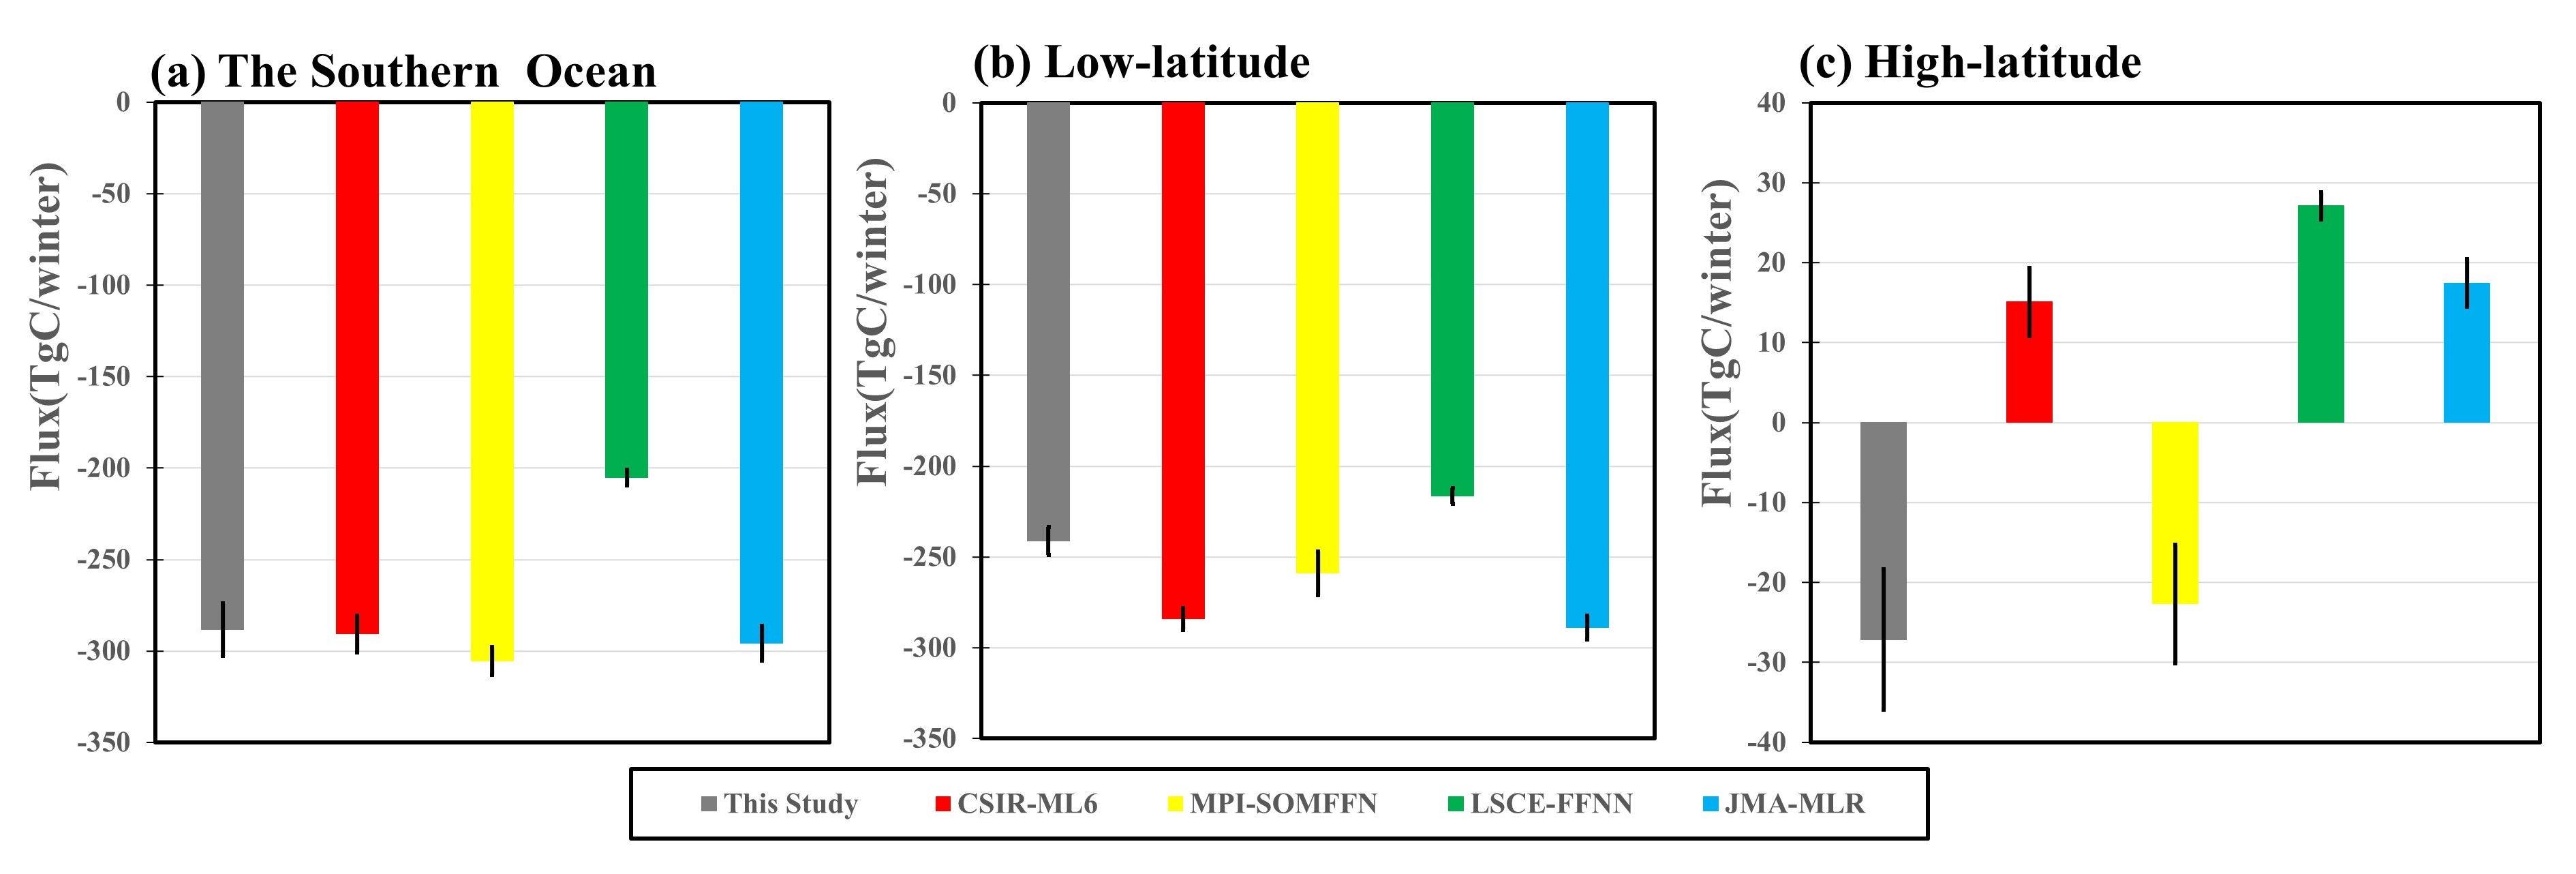
\includegraphics[width=\linewidth]{figure/第四章用图/图4-冬季平均.jpg}
    \bicaption{\label{fig:fig-4冬季平均}(a) 各产品冬季(5,6,7月)南大洋平均$\mathrm{CO_2}$通量(负数表示为$\mathrm{CO_2}$汇);(b)和(c) 分别为低纬度区域和高纬度区域各产品冬季平均$\mathrm{CO_2}$通量。}
    {(a) Average $\mathrm{CO_2}$ flux (negative number indicates $\mathrm{CO_2}$ absorption) in the Southern Ocean for each product during winter (May, June, July)  (b) and (c) are the average $\mathrm{CO_2}$ fluxes for each product in the low-latitude and high-latitude regions, respectively, during winter.}
\end{figure}
在以往的研究中多次提到了南大洋区域可能存在着分歧或者较大的不确定性,在我们对比的几种产品中,也看到了类似的现象;我们统计了多年来南大洋海气$\mathrm{CO_2}$交换通量的平均值,如\autoref{fig:fig-4冬季平均}所示。

在对比的四种产品中,可以发现LSCE-FFNN产品计算得到的$\mathrm{CO_2}$ flux量吸收最低,其他产品都基本在-280 TgC winter$^{-1}$左右。在低纬度和高纬度的对比中,明显能够看到差异最大在高纬度地区,多种产品表现并不一致。其中CSIR-ML6、LSCE-FFNN、JMA-MLR产品均认为南大洋冬季地区为碳源,分别 15.1±4.23、27.1±1.68和 17.5±2.97 TgC winter$^{-1}$;而使用忽略Chl-a处理策略的MPI-SOMFFN产品结果很出乎意料,认为是碳汇,其计算得到的$\mathrm{CO_2}$ 通量为 -22.7±7.43TgC winter$^{-1}$。而我们的结果认为,南大洋冬季应该是为碳汇地区,其碳汇通量为-27.1 ± 8.81 Tg C。

与其他产品的对比,可以发现使用了假设方法的产品多数低估了南大洋冬季$\mathrm{CO_2}$的吸收能力,即高估了冬季南大洋高纬度的$p\mathrm{CO_2}$,从\autoref{fig:fig-4pCO2空间分布}可以看出,多数产品在近南极大陆附近高估。过去的研究和基于浮标数据的推算均表明,受到西风和富含营养和无机碳的深层水影响,南极峰(Antarctic front, AF)以南的地区应为碳源区。且在Long等人\cite{long2021strong}基于九条飞行数据发现南大洋45°S以南应该是更接近于吸收排放平衡的中性区域。Arteaga等人\cite{arteaga2020seasonal}和Uchida等人\cite{uchida2019southern}发现在接近南极洲附近的海域的早冬时期可能存在着浮游植物爆发的现象,这可能与各种产品的假设相违背,导致了最后的估测误差。再结合MPI-SOMFFN产品冬季碳汇分布图(\autoref{fig:fig-4flux空间变化}),发现其产品高纬度区域,特别是接近ICE区域均为强碳汇区,这与已知的事实相悖,对其产品的结果表示存疑。综上所述,排除不确定性较大的MPI-SOMFFN产品,多数产品均认为冬季区域为碳源区,低估了南大洋冬季的吸收能力。

\section{本章小结}

本章一开始先介绍了目前的一些基于遥感回归方法的研究成果,并对每种产品进行介绍和分析。他们的成果对我们了解全球$p\mathrm{CO_2}$变化有着重要的作用,排除其他参数的影响,我们计算了这些产品的碳汇分布情况。接着利用第三章得到的模型进行反演南大洋月平均$p\mathrm{CO_2}$,能够发现南大洋的$p\mathrm{CO_2}$多年来以1.8μatm yr$^{-1}$的速度增长,但是略小于大气$p\mathrm{CO_2}$的增长速度(2.02 μatm yr$^{-1}$),表明南大洋吸收$\mathrm{CO_2}$的量可能在逐渐增加;$p\mathrm{CO_2}$在空间和时间尺度上有着显著的特点,如春夏季节的“双环结构”,以及在夏季低、冬季高的季节性变化,这与众多产品结果表现一致,但是从空间部分上来看仍有一些地方存在差异,其中差异最为显著的是冬季高纬度区域。

接着,结合空气传输速度我们计算出了各个产品的的海-气$\mathrm{CO_2}$交换通量,用于探究不同Chl-a处理策略下南大洋碳汇的碳汇的差异。从结果可以看出,整个南大洋碳汇量在研究时间内以0.016PgC\ yr$^{-1}$的速度在逐渐增长,从总量上来看,整个区域年平均吸收1.37±0.04PgC yr$^{-1}$,其中低纬度是主要吸收区,吸收了约0.96±0.02PgC yr$^{-1}$;而高纬度地区吸收了约0.35±0.03PgC yr$^{-1}$。从各个产品的对比来看,多数产品在高纬度的差异最大,除了与现有研究结果相悖的MPI-SOMFFN产品外,大多数产品再该区域表现为高估了$p\mathrm{CO_2}$,最终导致了整个高纬度区域的碳汇量低估。

总的来说,我们利用了基于主动遥感卫星的CALIPSO卫星的$b_{bp}$数据得到的结果表明,南大洋在冬季高纬度地区为碳汇区域,然而近些年使用不同Chl-a处理策略的产品大多数低估了南大洋冬季的碳汇。










